\chapter{Proposed System Design}
\section{Algorithm and Process Flow Model}

\begin{figure}[htpb]
\centering
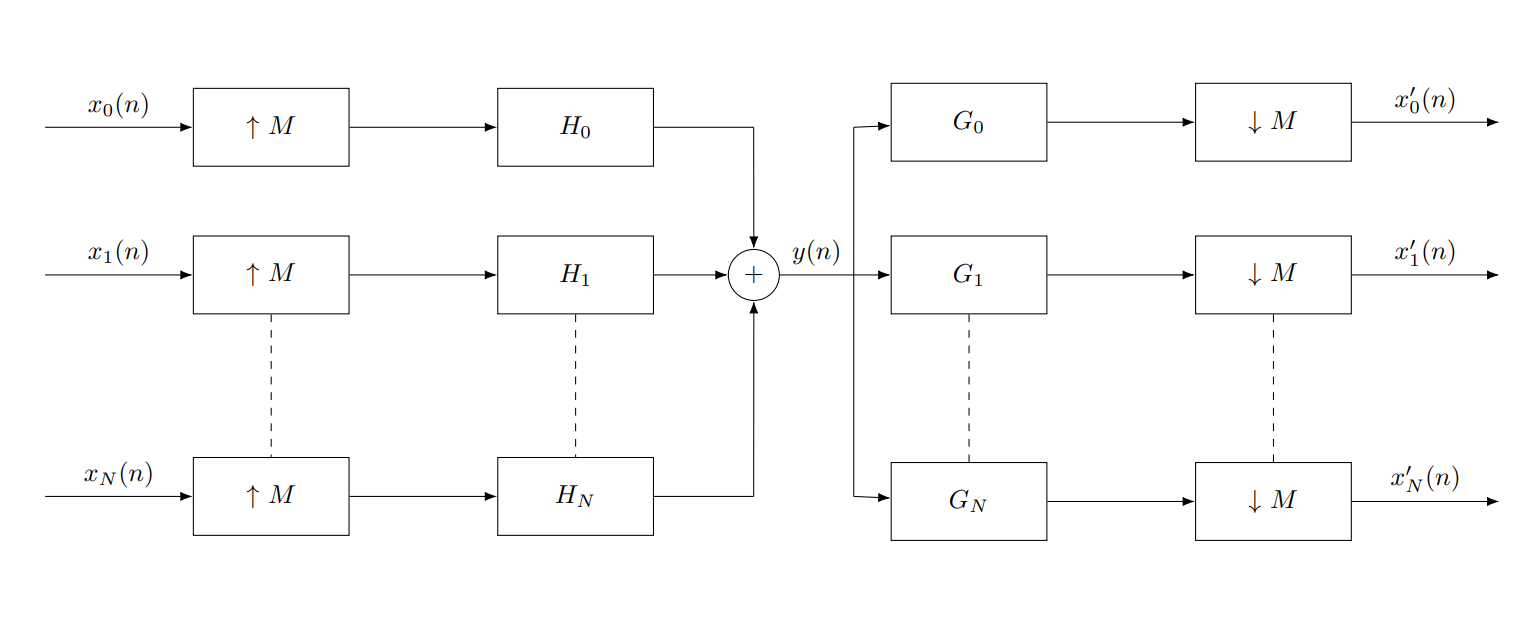
\includegraphics[width=5.2in]{system_block.png}
\caption{Block diagram of the System.}
\label{block}
\end{figure}

The design of Wavelet Transform based filters for a near Perfect Reconstruction (PR) Trans-multiplexer can be be explained in four steps \cite{b2} \cite{b5} \cite{b9}:
\begin{enumerate}
    \item Selection of a generic polynomial $T_{i,j}(z)$ based on the desired frequency response that satisfies the equation: 
\[ 
\frac{1}{2}[T_{i,j}(z) + T_{i,j}(-z)] = \left\{
  \begin{array}{lr} 
      z^{-2k}, & i = j, \\
      0, & i \neq j. 
      \end{array}
\right.
\]
Where, $T_{i,j} = H_i(z) G_j^T(z)$ i.e. product of the Z-Transform of the filter coefficients. $T_{i,j}$ is the Transmission polynomial, $H_i$ is the Synthesis filter, and $G_j$ is the Analysis filter.
\item Factorization of the polynomial $T_{i,j}(z)$ into $H_i(z)$ and $G_j(z)$, such that $H_i(z)$ contains all zeros only at $z = -1$. The degree of these polynomials is given by $(2N+1)$.
\item Using the generated inversion matrix of $H_i(z)$ and $G_j(z)$, choose the synthesis and analysis filters as elements of the co-factor matrix such that the determinant results in pure delay, leading to perfect reconstruction. 
\item Determination of the impulse responses of $H_i(z)$ and $G_j(z)$ for filter realization through the ``alternating signal'' construction.
\end{enumerate}
Fig. \ref{block} shows the block diagram of the system with the synthesis and analysis filters represented as defined, with the frequency factor $M$.


\section{Designed System}
The following system design was conducted based on given specifications for 3  input signals ($N = 3$). These include 2 voice signals in the band of 20 Hz - 4 kHz and 1 for metadata in the band of 300 Hz - 3.4 kHz. The same algorithm can be extended to include more number of signals in other frequency bands. The frequency factor $M$ was chosen as 4. Using the above algorithm, the resulting filters for analysis and synthesis steps are as follows:

\[ 
 H_0(z) = 1.479  + 6.7842 z^{-1} + 3.5243 z^{-2} - 0.2656 z^{-3} - 1.775 z^{-4} + 0.292 z^{-5} + 0.3121 z^{-6} - 0.106 z^{-7}
\]
\[
H_1(z) = 0.2304 + 0.715 z^{-1} + 0.631 z^{-2} - 0.028 z^{-3} - 0.187 z^{-4} + 0.039 z^{-5} + 0.033 z^{-6} - 0.497 z^{-7}
\]
\[
H_2(z) = 2.186 + 6.784 z^{-1} + 5.9487 z^{-2} - 0.2656 z^{-3} - 1.775 z^{-4} + 0.2927 z^{-5} + 0.311 z^{-6} + 1.244z^{-7}
\]
\[ 
 G_0(z) = -0.0942 + 0.292 z^{-1} + 0.276 z^{-2} - 1.674 z^{-3} - 0.2504 z^{-4} + 1.143 z^{-5} + 6.396 z^{-6} + 2.061 z^{-7}
\]
\[ 
 G_1(z) = -0.017 + 0.039 z^{-1} + 0.0384 z^{-2} - 0.187 z^{-3} - 0.028 z^{-4} + 0.631 z^{-5} + 0.718 z^{-6} + 0.231 z^{-7}
\]
\[
G_2(z) =  1.203 + 0.292 z^{-1} + 0.226 z^{-2} - 1.6744 z^{-3} - 0.254 z^{-4} + 5.983 z^{-5} + 6.346 z^{-6} + 1.823 z^{-7}
\]

The resultant frequency response of the designed filters is shown in Fig. \ref{freq_resp}. The phase response of the designed filters is shown in Fig. \ref{phase_resp}.

\begin{figure}[htpb]
\centering
\begin{tabular}{cc}
  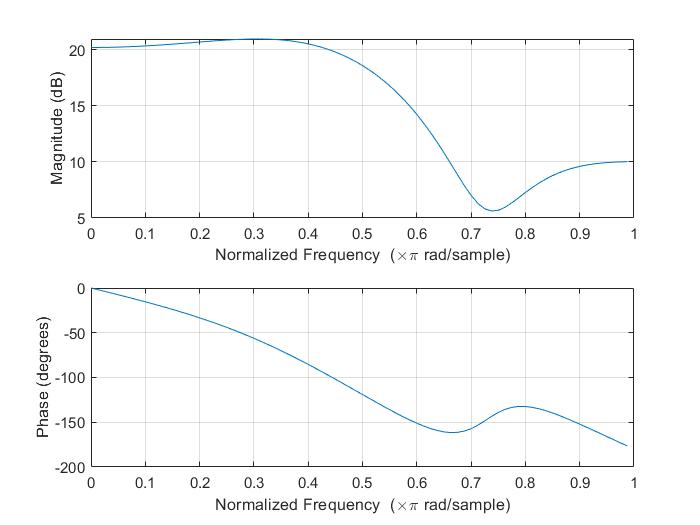
\includegraphics[trim={0 9cm 0 0}, clip, width=75mm]{H0.jpg} & 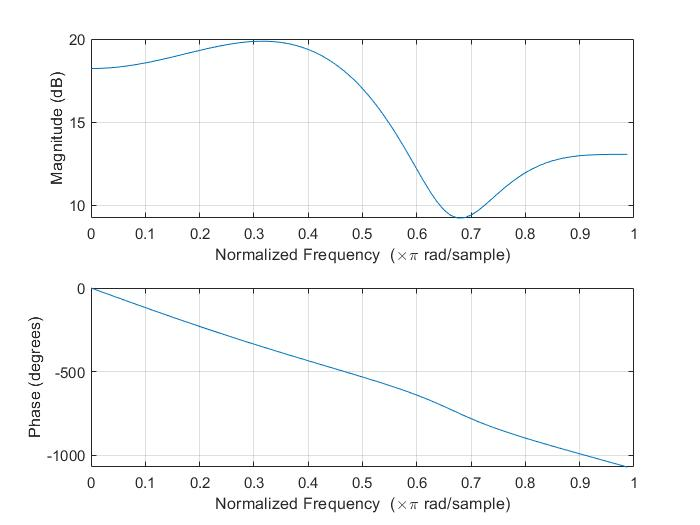
\includegraphics[trim={0 9cm 0 0}, clip,width=75mm]{G0.jpg} \\
(a) Synthesis filter $H_0$ & (b) Analysis filter $G_0$ \\[6pt]
 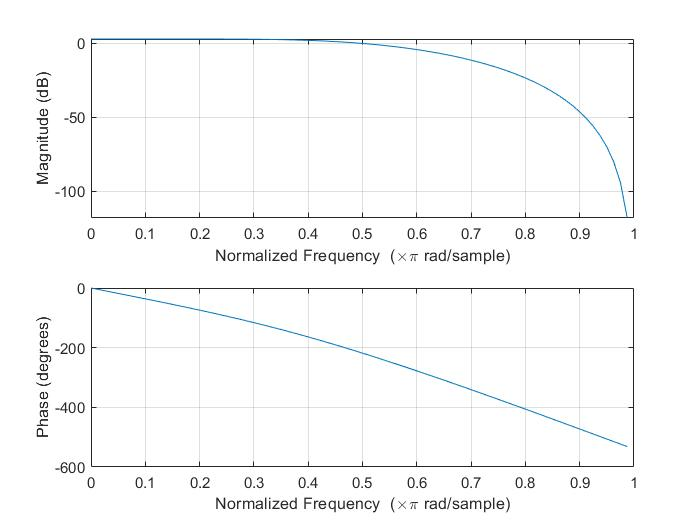
\includegraphics[trim={0 9cm 0 0}, clip,width=75mm]{H1.jpg} & 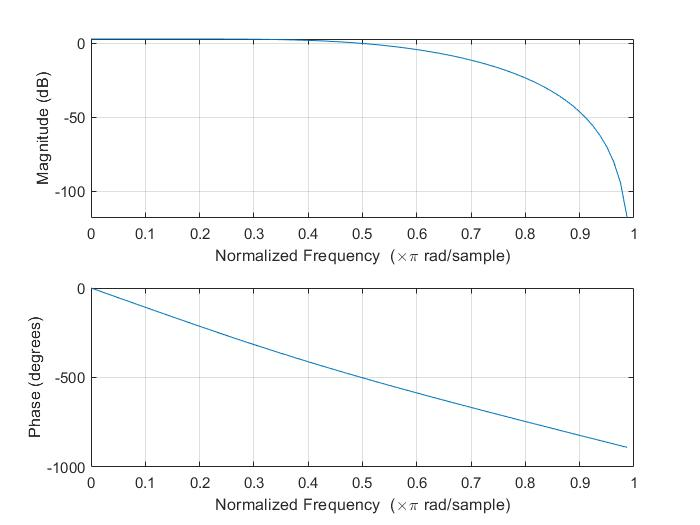
\includegraphics[trim={0 9cm 0 0}, clip,width=75mm]{G1.jpg} \\
(c) Synthesis filter $H_1$  & (d) Analysis filter $G_1$  \\
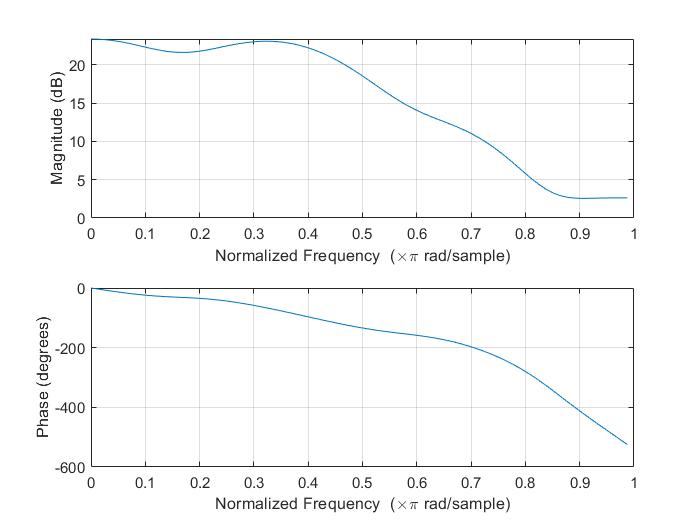
\includegraphics[trim={0 9cm 0 0}, clip,width=75mm]{H2.jpg} & 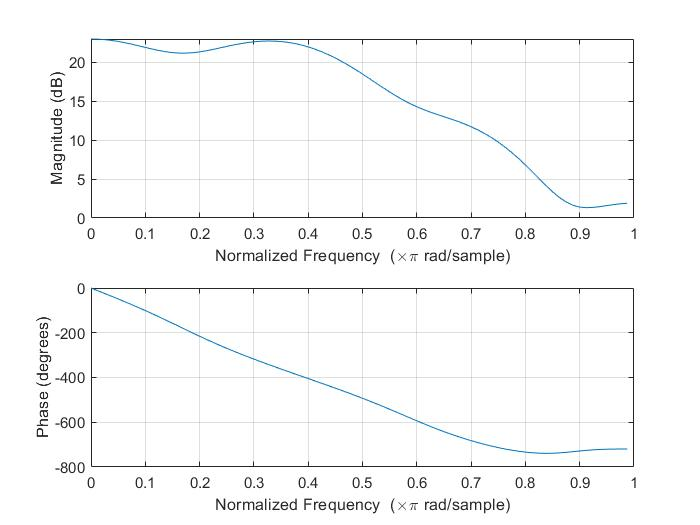
\includegraphics[trim={0 9cm 0 0}, clip,width=75mm]{G2.jpg} \\
(e) Synthesis filter $H_2$ & (f) Analysis filter $G_2$\\[6pt]
\end{tabular}
\caption{Frequency response plots of the designed filters.}
\label{freq_resp}
\end{figure}

\begin{figure}[htpb]
\centering
\begin{tabular}{cc}
  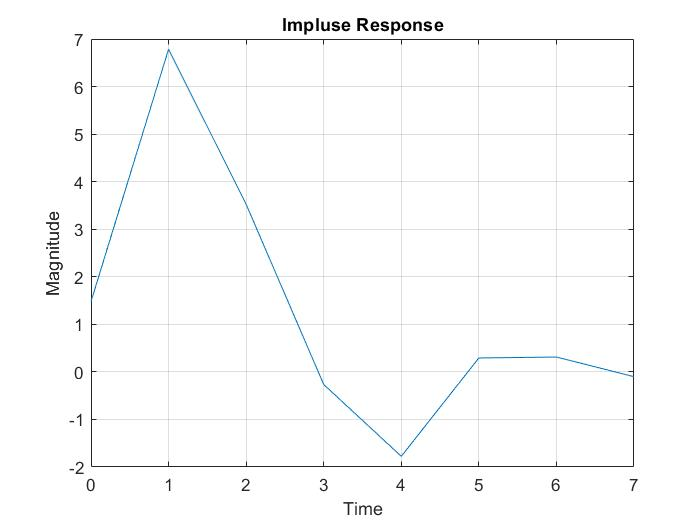
\includegraphics[width=75mm]{H0_Response.jpg} & 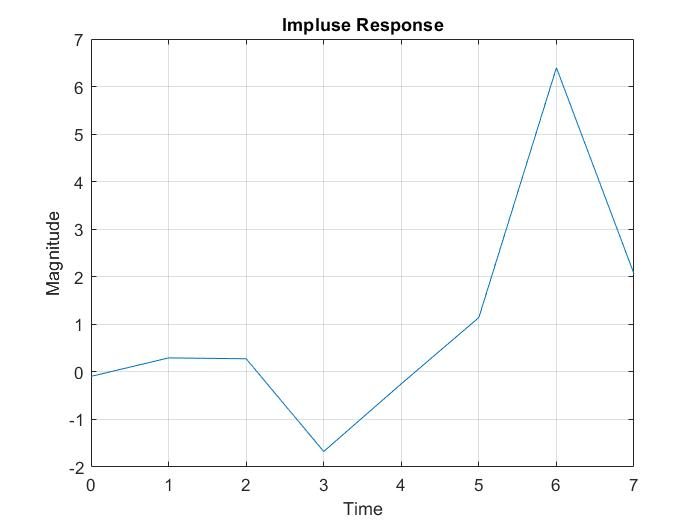
\includegraphics[width=75mm]{G0_Response.jpg} \\
(a) Synthesis filter $H_0$ & (b) Analysis filter $G_0$ \\[8pt]
 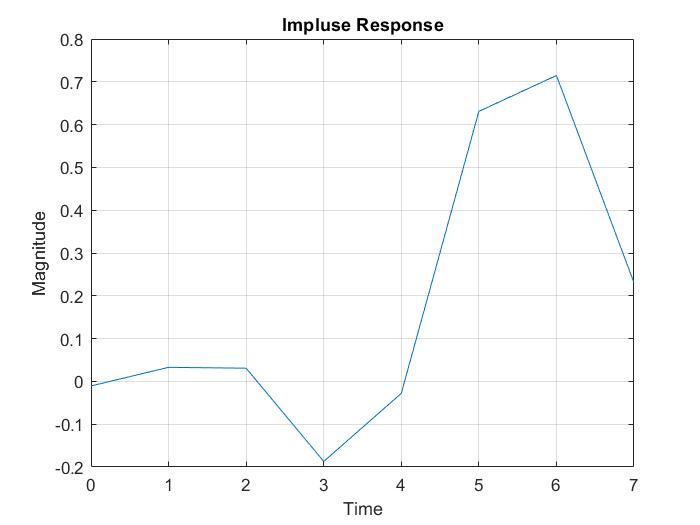
\includegraphics[width=75mm]{H1_Response.jpg} & 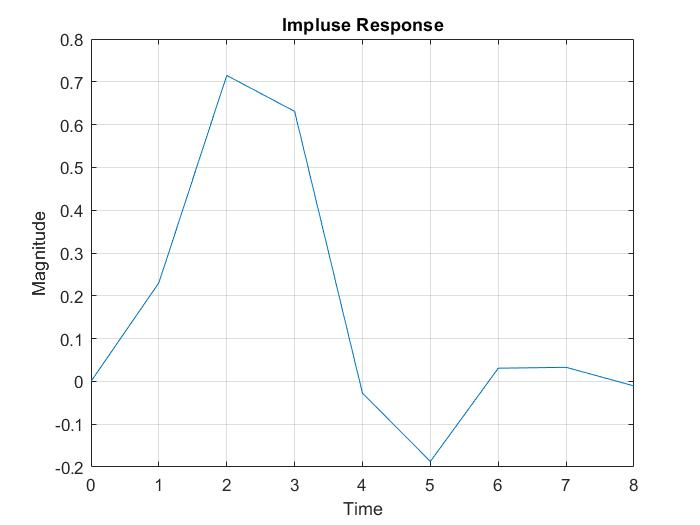
\includegraphics[width=75mm]{G1_Response.jpg} \\
(c) Synthesis filter $H_1$  & (d) Analysis filter $G_1$  \\ [8pt]
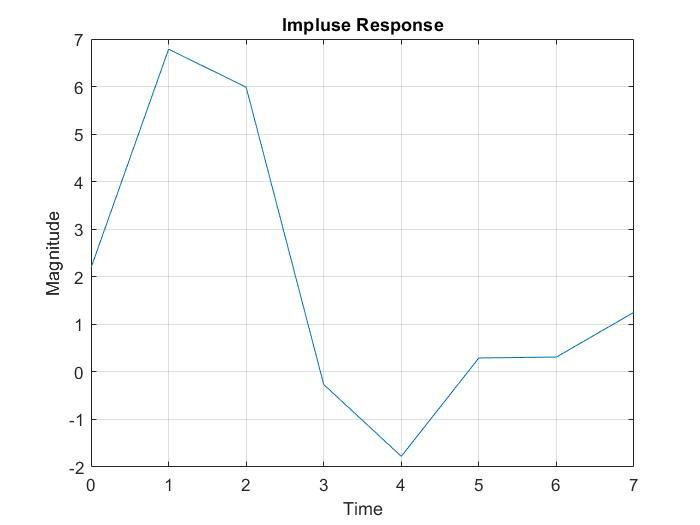
\includegraphics[width=75mm]{H2_Response.jpg} & 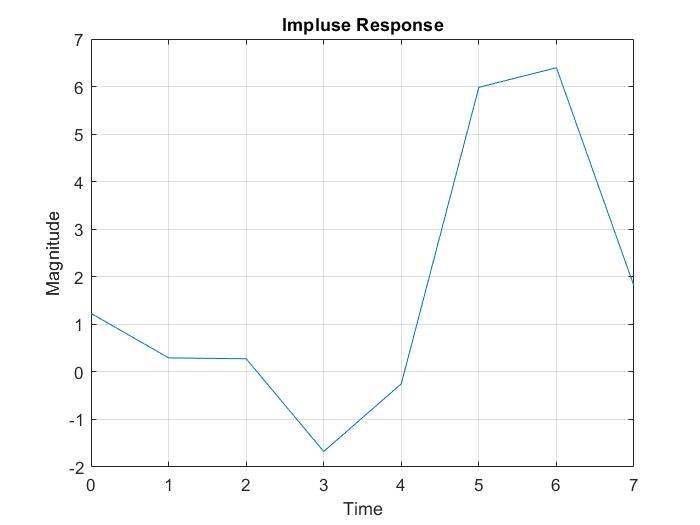
\includegraphics[width=75mm]{G2_Response.jpg} \\
(e) Synthesis filter $H_2$ & (f) Analysis filter $G_2$\\[8pt]
\end{tabular}
\caption{Impulse response plots of the designed filters.}
\label{imp_resp}
\end{figure}

\begin{figure}[htpb]
\centering
\begin{tabular}{cc}
  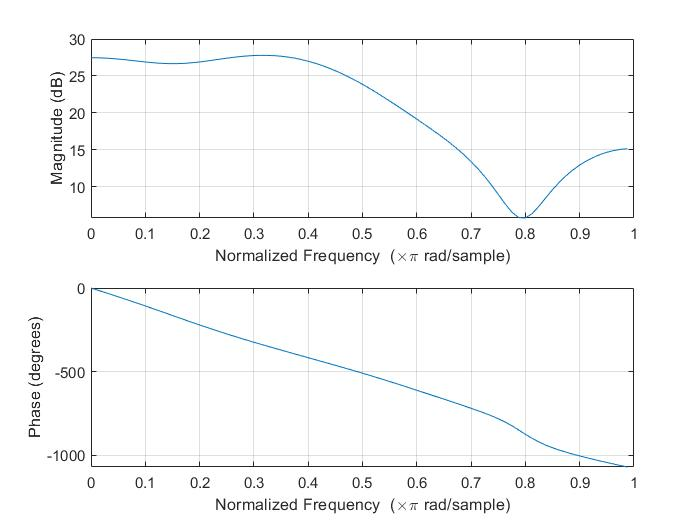
\includegraphics[width=80mm]{H_System.jpg} & 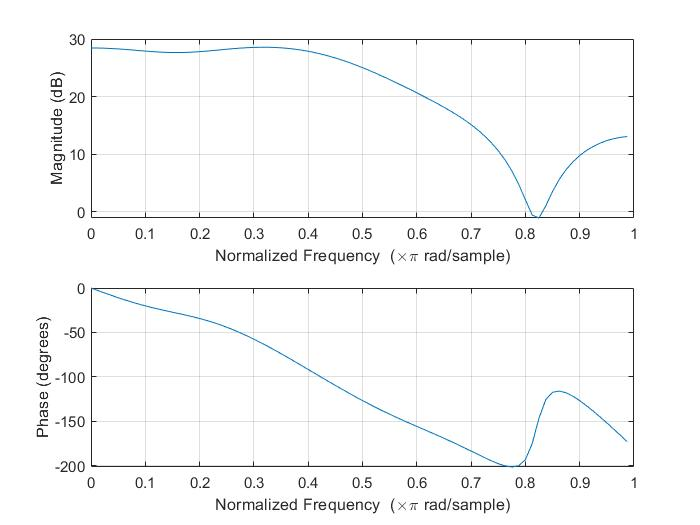
\includegraphics[width=80mm]{G_System.jpg} \\ [10pt]
(a) Synthesis filter response  & (b) Analysis filter response \\[10pt]
%  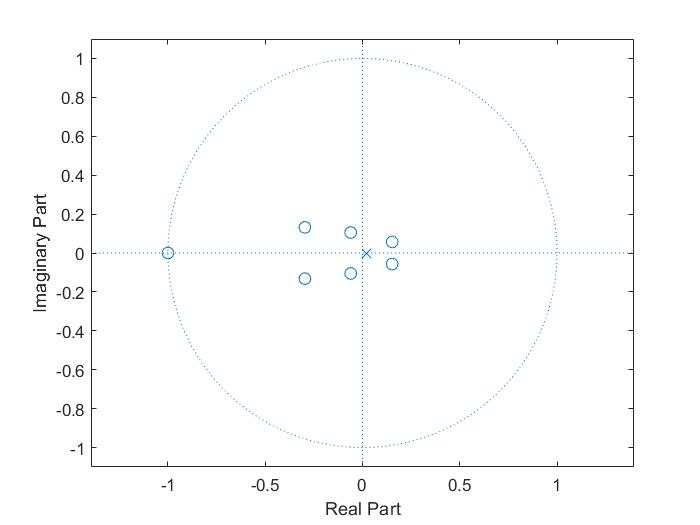
\includegraphics[width=75mm]{H_System_pzmap.jpg} & 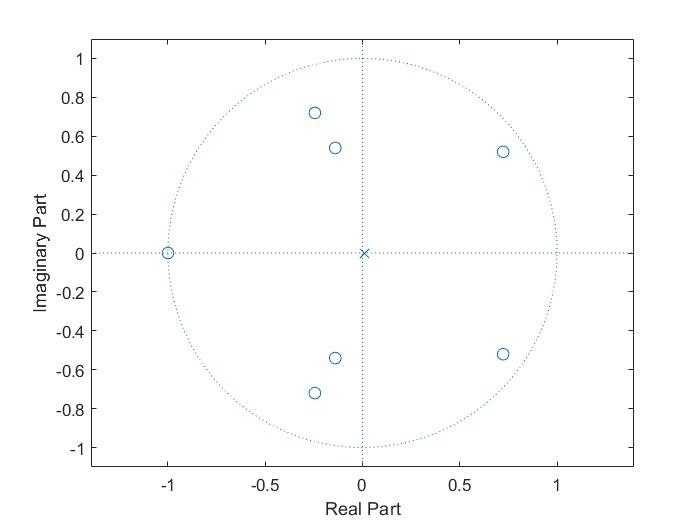
\includegraphics[width=75mm]{G_System_pzmap.jpg} \\ [8pt]
% (c) Synthesis filter pole-zero plot & (d) Analysis filter pole-zero plot \\
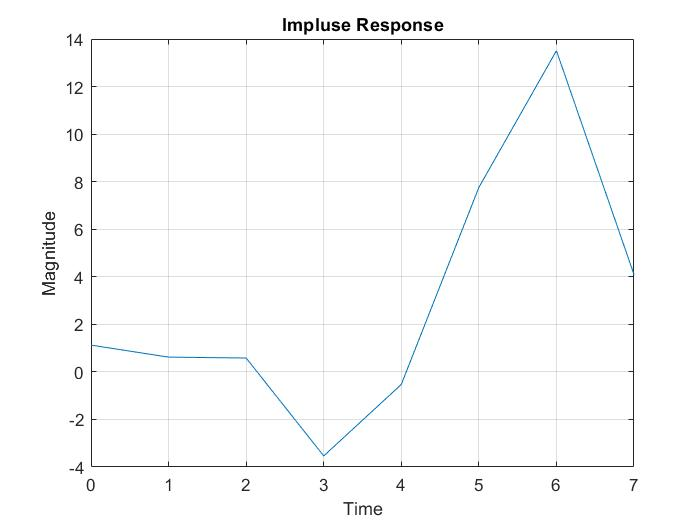
\includegraphics[width=80mm]{H_System_Response.jpg} & 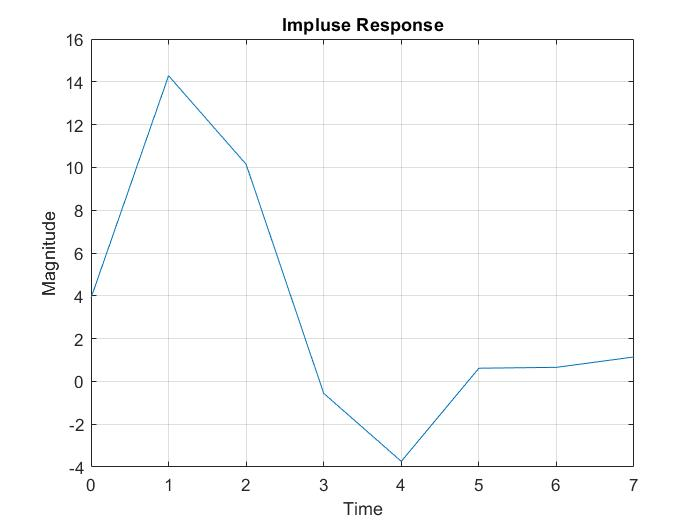
\includegraphics[width=80mm]{G_System_Response.jpg} \\ [10pt]
(c) Synthesis filter impulse response & (d) Analysis filter impulse response\\[10pt]
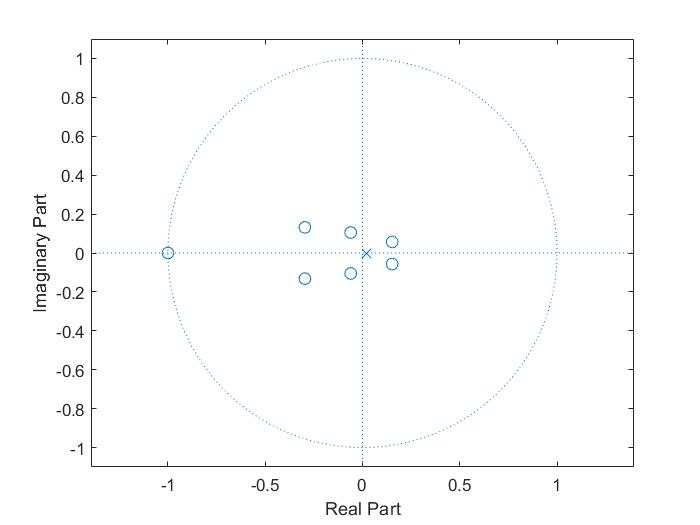
\includegraphics[width=80mm]{H_System_pzmap.jpg} & 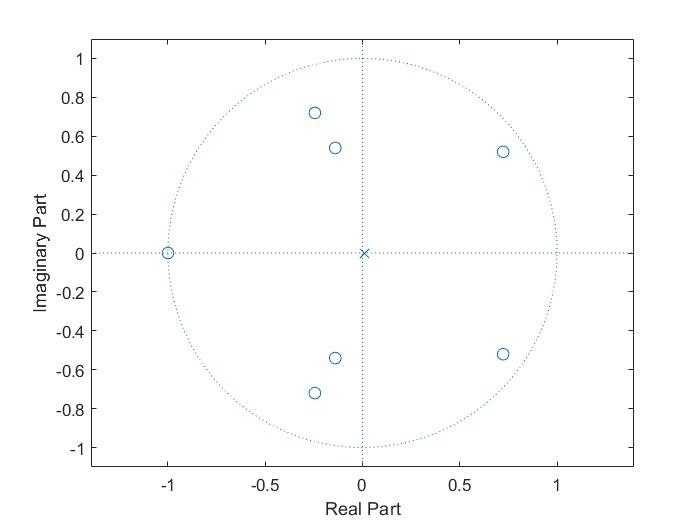
\includegraphics[width=80mm]{G_System_pzmap.jpg} \\ [10pt]
(c) Synthesis filter Pole-zero Map & (d) Analysis filter Pole-zero Map\\[10pt]
\end{tabular}
\caption{Aggregated response plots of the system.}
\label{system}
\end{figure}

\newpage

% The matrix form of the system is as follows: \par
% 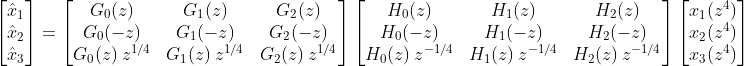
\includegraphics[width=175mm]{matrix_eqn.png}

\begin{figure}[htpb]
\centering
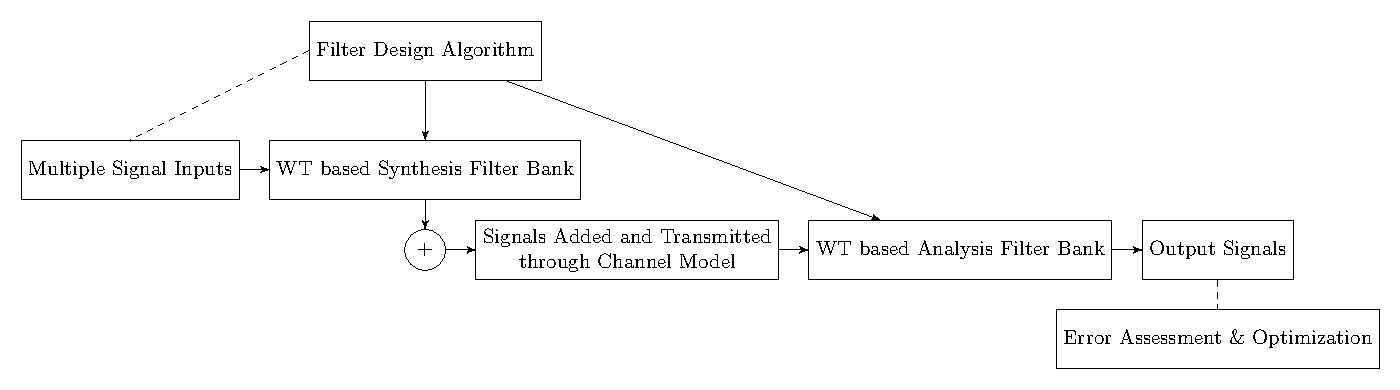
\includegraphics[width=5.95in]{process_flow.pdf}
\caption{Flow diagram of the System.}
\label{flow}
\end{figure}

From the frequency response plots of the designed filters, it is seen that filters $H_0$ and $G_0$ are low pass filters, which correspond to the channel requirements of the metadata signal. The remaining filters are have higher cut-offs to meet the specifications of the voice signals. The plots are similar to those obtained in \cite{b2} \cite{b5}, thus verifying the design. After the filters are designed to meet the specifications, they can be incorporated in the WT-based filter bank as a part of the Trans-multiplexer system. Fig. \ref{flow} shows the overall flow of the designed system. The multiple signal inputs are then individually fed into the synthesis part of the system, where the filter bank performs the relevant processing. The processed signals are then added (concatenated) to be transmitted through the chosen channel model. In the receiver section, the received signal passes through the analysis part of the system, where the signals are perfectly reconstructed into their constituent parts. The output signals are then compared with the original input signals for error analysis and optimization of the system.

\begin{figure}[htpb]
\centering
\begin{tabular}{cc}
  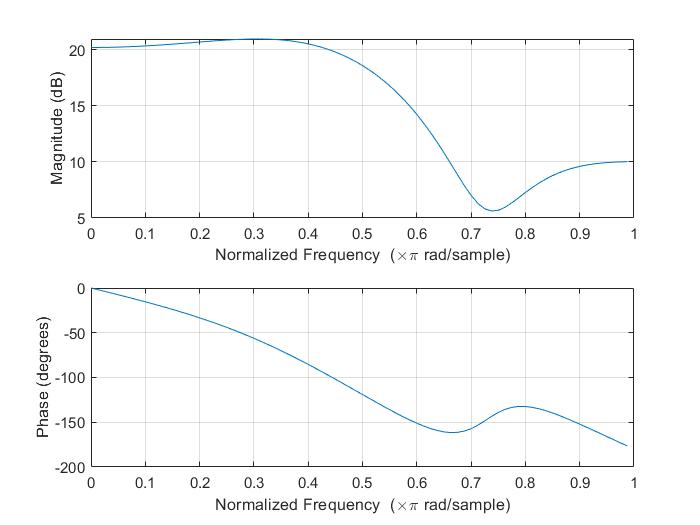
\includegraphics[trim={0 0 0 9.3cm}, clip, width=75mm]{H0.jpg} & 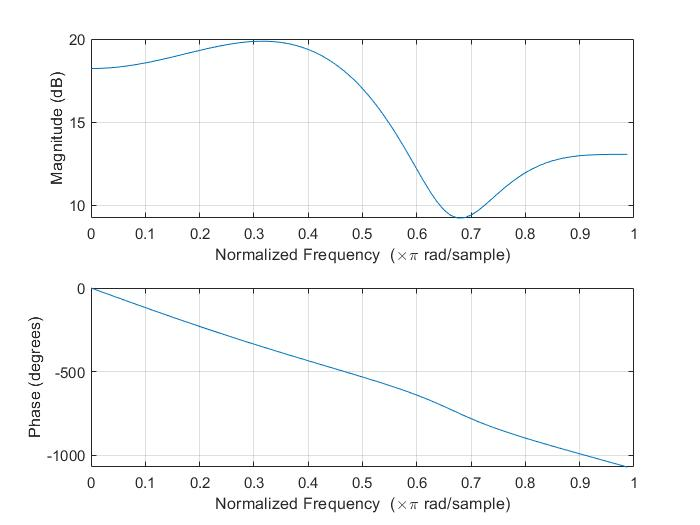
\includegraphics[trim={0 0 0 9.3cm}, clip,width=75mm]{G0.jpg} \\
(a) Synthesis filter $H_0$ & (b) Analysis filter $G_0$ \\[6pt]
 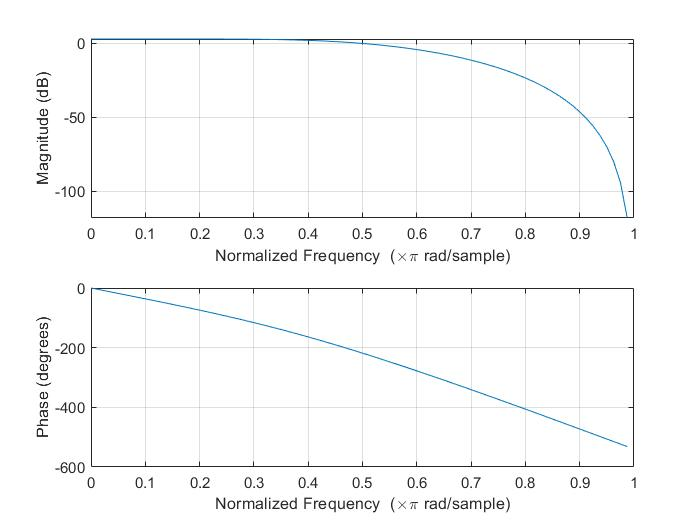
\includegraphics[trim={0 0 0 9.3cm}, clip,width=75mm]{H1.jpg} & 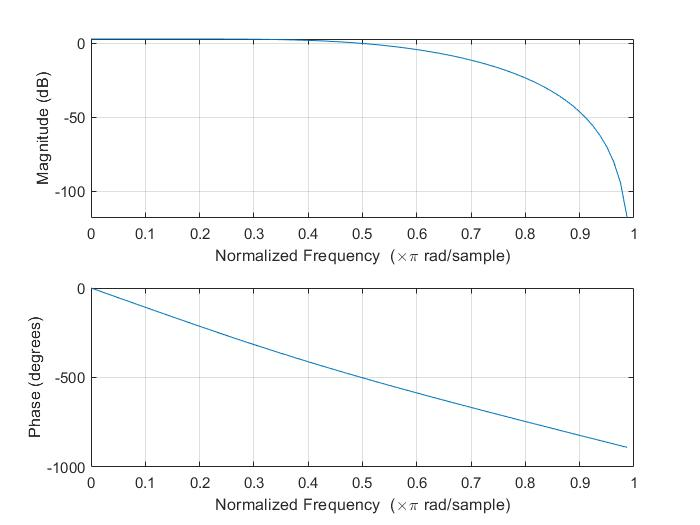
\includegraphics[trim={0 0 0 9.3cm}, clip,width=75mm]{G1.jpg} \\
(c) Synthesis filter $H_1$  & (d) Analysis filter $G_1$  \\
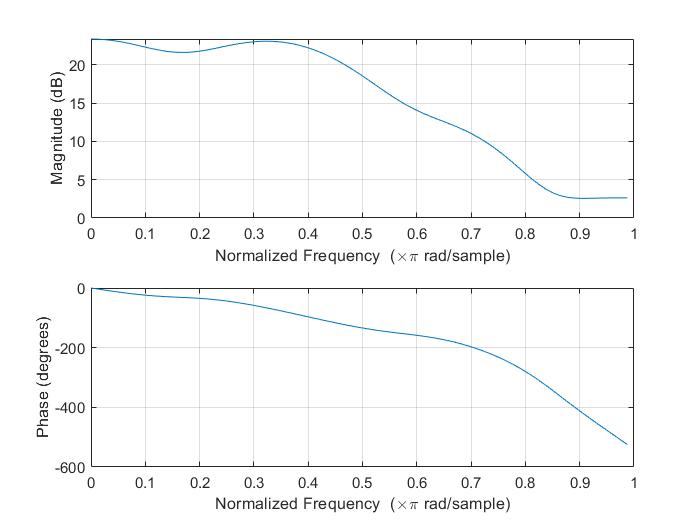
\includegraphics[trim={0 0 0 9.3cm}, clip,width=75mm]{H2.jpg} & 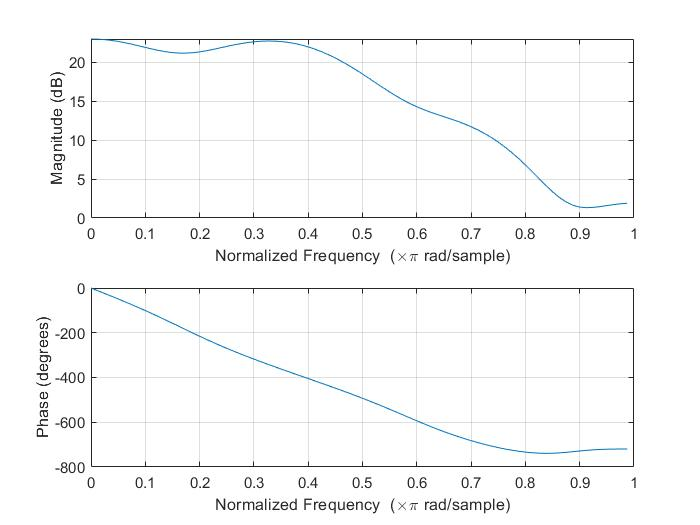
\includegraphics[trim={0 0 0 9.3cm}, clip,width=75mm]{G2.jpg} \\
(e) Synthesis filter $H_2$ & (f) Analysis filter $G_2$\\[6pt]
\end{tabular}
\caption{Phase response plots of the designed filters.}
\label{phase_resp}
\end{figure}


\section{Implementation using MATLAB}
This section describes the realization of the designed filters and the Trans-multiplexer system as described above using MATLAB \cite{b20}. The designed filter parameters are imported, and the input signals are defined. The WT-based \textit{DWTAnalysisFilterBank} and \textit{DWTSynthesisFilterBank} objects are then defined using the relevant designed filters. These objects accept the `$NumLevels$' parameter i.e. the frequency factor $M = 4$ for the selected case. The `$Filter$' parameter can also be specified, which changes the wavelet family of the mother wavelet used to perform the transforms. These parameters will help in the testing and optimization of the system. The input signals are then passed through the \textit{DWTSynthesisFilterBank} object and are then added and transmitted over the channel model. The received signal is then passed through the \textit{DWTAnalysisFilterBank} object to reconstruct the original signals. The original, reconstructed, and error signals are then plotted on the scope, and the mean system error is calculated to evaluate system performance. 



 \begin{figure}[htpb]
\centering
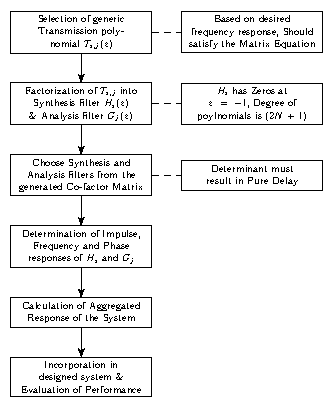
\includegraphics[width = 5in]{Design_algorithm.pdf}
\caption{Flow diagram of the algorithm.}
\label{algo}
\end{figure}

